%Dies ist die Hauptseite des Dokumentes. Es werden u. a. alle Kapitel,
%Einstellung im Header eingebunden.  Veränderungen müssen in folgenden Dateien
%vorgenommen werden:
      %- Layout.tex
      %- newComments.tex
      %- Titelseite
      %- Versionsübersicht
      %- einzelne Kapitel (evtl. erweitern)


% Definition von globalen Parametern, die derzeit auf der Titelseite und in der
% Kopfzeile verwendet werden. Der in <> gesetzte Text ist zu verändern.

\newcommand{\praktikumTitel}{<Titel des Praktikums>}
\newcommand{\projektTitel}{<Titel des Teilprojektes>}


%Hier sind alle Einstellungen enthalten, die sich auf das Seiten- und
%Dokumentenlayout beziehen

\documentclass[
  11pt,                % Schriftgröße
  DIV12,
  german,              % für Umlaute, Silbentrennung etc.
  oneside,             % einseitiges Dokument
  titlepage,           % es wird eine Titelseite verwendet
  halfparskip,         % Abstand zwischen Absätzen (halbe Zeile)
  normalheadings,      % Größe der Überschriften verkleinern
  tablecaptionabove,   % Beschriftung von Tabellen unterhalb ausgeben
  final                % Status des Dokuments (final/draft)
]{scrreprt}            %


%------Ändern von Schriftschnitten - (Muss ganz am Anfang stehen !) ------------
\usepackage{fix-cm}

%------Umlaute -----------------------------------------------------------------
%   Umlaute/Sonderzeichen wie äüöß können direkt im Quelltext verwenden werden.
%    Erlaubt automatische Trennung von Worten mit Umlauten.
\usepackage[T1]{fontenc}
\usepackage[utf8]{inputenc}

%------Anpassung der Landessprache----------------------------------------------
\usepackage{ngerman}

%------Einfache Definition der Zeilenabstände und Seitenränder------------------
\usepackage{geometry}
\usepackage{setspace}

%------Schriftgrößenanpassung von einzelnen Textpassagen------------------------
\usepackage{relsize}

%------Trennlinien in Kopf- und Fusszeile
\usepackage[headsepline, footsepline, ilines]{scrpage2}

%------Grafiken-----------------------------------------------------------------
\usepackage{graphicx}

%------Packet zum Sperren, Unterstreichen und Hervorheben von Texten------------
\usepackage{soul}

%------ergänzende Schriftart----------------------------------------------------
\usepackage{helvet}

%------Lange Tabellen-----------------------------------------------------------
\usepackage{longtable}
\usepackage{array}
\usepackage{ragged2e}
\usepackage{lscape}

%------PDF-Optionen-------------------------------------------------------------
\usepackage[
  bookmarks,
  bookmarksopen=true,
  colorlinks=true,
  linkcolor=black,        % einfache interne Verknüpfungen
  anchorcolor=black,      % Ankertext
  citecolor=black,        % Verweise auf Literaturverzeichniseinträge im Text
  filecolor=black,        % Verknüpfungen, die lokale Dateien öffnen
  menucolor=black,        % Acrobat-Menüpunkte
  urlcolor=black,         % Farbe für URL-Links
  backref,                % Zurücktext nach jedem Bibliografie-Eintrag als
                          % Liste von Überschriftsnummern
  pagebackref,            % Zurücktext nach jedem Bibliografie-Eintrag als
                          % Liste von Seitenzahlen
  plainpages=false,       % zur korrekten Erstellung der Bookmarks
  pdfpagelabels,          % zur korrekten Erstellung der Bookmarks
  hypertexnames=false,    % zur korrekten Erstellung der Bookmarks
  linktocpage             % Seitenzahlen anstatt Text im Inhaltsverzeichnis
                          % verlinken
  ]{hyperref}



      % enthält eingebundene Packete

%------Seitenränder-------------------------------------------------------------
\geometry{verbose,                     % zeigt die eingestellten Parameter beim
                                       % Latexlauf an
      paper=a4paper,                   % Papierformat
      top=25mm,                        % Rand oben
      left=25mm,                       % Rand links
      right=25mm,                      % Rand rechts
      bottom=45mm,                     % Rand unten
      pdftex                           % schreibt das Papierformat in die
                                       % Ausgabe damit Ausgabeprogramm
                                       % Papiergröße erkennt
  }

%Seitenlayout
\onehalfspace        % 1,5-facher Abstand

%------Kopf- und Fußzeilen -----------------------------------------------------
\pagestyle{scrheadings}

%------Kopf- und Fußzeile auch auf Kapitelanfangsseiten ------------------------
\renewcommand*{\chapterpagestyle}{scrheadings}

%------Schriftform der Kopfzeile -----------------------------------------------
\renewcommand{\headfont}{\normalfont}

%------Kopfzeile----------------------------------------------------------------
\setlength{\headheight}{21mm}        % Höhe der Kopfzeile
\ihead{\large{\textsc{\praktikumTitel}}\\    % Text in der linken Box
       \small{\projektTitel}}
\chead{}                             % Text in der mittleren Box

%----Fusszeile
\cfoot{}                             % Text in mittlerer Box
\ofoot{\pagemark}                    % Seitenzahl in rechter Box

          % Diese Datei enthält alle
                                          % Layouteinstellungen

%------Beginn des Gesamtdokumentes----------------------------------------------
\begin{document}

%------Eingebundene Seiten, Verzeichnisse bzw. Kapitel--------------------------
\include{titelseite}                      % Titelseite
%Diese Datei dient der Versionskontrolle. Sie ist vollständig zu bearbeiten.

%----Überschrift------------------------------------------------------------
{\relsize{2}\textbf{Versionsübersicht}}\\[2ex]

%----Start der Tabelle------------------------------------------------------
\begin{longtable}{|m{1.78cm}|m{1.59cm}|m{2.86cm}|m{1.9cm}|m{5.25cm}|}

  \hline                                              % Linie oberhalb

  %----Spaltenüberschriften------------------------------------------------
  \textbf{Version}  &    \textbf{Datum}  &    \textbf{Autor}  &
  \textbf{Status}   &    \textbf{Kommentar}  \\       %Spaltenüberschrift
  \hline                                              % Gitterlinie

  %----die nachfolgeden beiden Zeilen so oft wiederholen und die ... mit den
  %i   entsprechenden Daten zu füllen wie erforderlich
  0.1  &   02.07.2011  & Simon Hahne    &   in Bearbeitung    &    Initialisierung\\       % Eintrag in Zeile
  \hline
	0.2  &    &    &   in Bearbeitung    &  \\       % Eintrag in Zeile
  \hline   
	0.3  &     &   &    in Bearbeitung    &   \\       % Eintrag in Zeile
  \hline   
	0.4  &    &   &   in Bearbeitung    &    \\       % Eintrag in Zeile
  \hline   
	0.5  &     &  &   in Bearbeitung    &    \\       % Eintrag in Zeile
  \hline   % Gitterlinie unten

%----Ende der Tabelle------------------------------------------------------
\end{longtable}
Status: "`in Bearbeitung"' oder "`abgenommen"'\\
Kommentar: hier eintragen, was geändert bzw. ergänzt wurde

       % Versionsübersicht

\tableofcontents                          % Inhaltsverzeichnis wird automatisch
                                          % generiert
\listoffigures                            % ebenso das Abbildungsverzeichnis

Abbildung 1: StateChart Projektdetails  5 \\
Abbildung 2: Verteilung von <ID>  7       \\
Abbildung 3: Sequenzdiagramm für <ID>  7  \\
Abbildung 4: Komponentendiagramm  8       \\
Abbildung 5: Protokollstatechart für jede Komponente  9    \\
Abbildung 6: Verteilungsdiagramm  10      \\




%----Kapitel des Feinentwurfs, die mit Inhalt zu füllen sind--------------------
% Kapitel 1
%-------------------------------------------------------------------------------


\chapter{Einleitung}
Wie in der Vorlesung erwähnt, ist das Testen von Software unerlässlich und darf
bei keinem Softwareentwicklungsprozess fehlen.

Diese Testdokumentation ist angelehnt an den IEEE 829-Standard, der als
der bekannteste -- wenn nicht sogar einzige -- Standard für Software-
Testdokumentationen gilt. Der Standard definiert eine Menge von Testdokumenten
und beschreibt deren Inhalte.                 % Kapitel 1
% Kapitel 2 mit den entsprechenden Unterkapiteln
% Die Unterkapitel können auch in separaten Dateien stehen,
% die dann mit dem \include-Befehl eingebunden werden.
%-------------------------------------------------------------------------------
\chapter{Analyse der Produktfunktionen}

%Die Kapitel müssen mit Inhalt gefüllt werden!. Eine Bereiche habe ich beuwsst schon bei der Verteildung der Diagramme zusammengefasst 
%In diesen Bereichen möchte ich euch bitten die jeweiligen Unterpunkte kurz mit den Oberpunkten zu vergleichen und zu argumentieren 
%warum es sich um triviale Spezialfälle handelt die keiner näheren beschreibung bedürfen
%
% Ich hab mal immer davon geschrieben welche Bereich von wem gemacht werden

\section{Analyse der Funktionalität /F100/: Spezifikation einlesen}
Das Einlesen einer Spezifikation aus einem vom Nutzer angegebenen Dateipfad
gliedert sich in mehrere Teilfunktionalitäten. Zunächst muss der Anwender den
Dateipfad auswählen. Dafür sollte ein Datei-Dialog zum Einsatz kommen.
Danach muss die ausgewählte Datei geöffnet, geprüft und geparst werden. Für
diese Aufgaben bietet sich eine spezialisierte Komponente an, um alle
Eigenheiten des Dateiformates von der Oberfläche und dem Simulator abzukapseln.
Der ausgelesene Datensatz wird nun zum Starten einer neuen Simulation verwendet,
dafür muss eine eventuell laufende Simulation beendet werden. Es bietet sich
an, diese Funktionen als Schnittstelle zu kapseln und die konkrete Implementierung
der Simulator-Komponente zu überlassen.

\begin{figure}[h!]
\includegraphics[width=\linewidth]{bilder/spezifikation_einlesen}
\caption{Sequenzdiagramm für \textit{Spezifikation einlesen}}
\end{figure}

%Christian/Matthias

%kann man dies ggf Q40 zuordnen?
\section{Analyse von Funktionalität :  Renderloop}
Da es sich um ein System handelt, in dem eine ständige Berechnung (Loop) zur Laufzeit notwendig wird, einerseits durch die 3D-Anzeige, die eine ständige Aktualisierung erwartet und andererseits durch
die Simulation an sich, ist es sinnig diesen Vorgang ebenfalls näher zu beleuchten.

\begin{figure}[h!]
\includegraphics[width=\linewidth]{bilder/render_loop}
\caption{Sequenzdiagramm für \textit{Renderloop}}
%\label{labelname}
\end{figure}

Der Simulator initiiert einen Simulationsschritt indem ein neuer Simulationsschritt bei der Simulation angefordert  wird. Die erhalten Daten werden dann zur 3D-Anzeige weitergereicht und werden dort visualisiert.

%Simon:
\section{Analyse von Funktionalität /F200/ :  Starten/Stoppen der Simulation}
Der Anwender kann über die GUI die Simulation starten. Dabei wird die Information an den Simulator weitergeleitet, der das 3D Bild anzeigt, die 2D Statusanzeige einblendet, die Bahnberechnung startet und die Aufzeichnung startet. 
Der Anwender kann außerdem über die GUI die Simulation stoppen. Dabei wird die Information ebenfalls an den Simulator weitergeleitet, der dann alles wieder schließt und die Aufzeichnung speichert.

<<<<<<< HEAD
\begin{figure}
\includegraphics[width=\linewidth]{bilder/Starten_Stoppen.pdf}
=======
\begin{figure}[h!]
\includegraphics[width=\linewidth]{bilder/Simulator_Starten_Stoppen}
>>>>>>> 1707a661acfb7fc7ebf6e25dc5e88812589d4610
\caption{Sequenzdiagramm für das \textit{Starten und Stoppen der Simulation}}
%\label{labelname}
\end{figure}

%Robin
\section{Analyse von Funktionalität /F300/ :  Pausieren der Simulation}
Der Anwender hat während der Simulation die Möglichkeit diese anzuhalten und sie später fortzusetzen, ohne dass die Pausierung Auswirkungen auf das Simulationsergebnis hat.
\newline

\begin{figure}[!h]
\includegraphics[viewport = 0 17.5cm 25cm 30cm, width=\linewidth]{bilder/Pausieren.pdf}
\caption{Sequenzdiagramm für \textit{Pausieren der Simulation}}
%\label{labelname}
\end{figure}

%Daniel
\section{Analyse von Funktionalität /F400o/ :  Video aufzeichnen}
Der Anwender kann über die GUI die Eingabe tätigen, ein Video aufzeichnen zu wollen, sofern nicht gerade eine Aufnahme läuft. Die GUI gibt diese Anweisung an die 3D-Anzeige weiter, die nun mit der
Videoaufnahme beginnt. Dies geschieht so lange, bis der Anwender die Videoaufzeichnung stoppt. In diesem Fall wird die Aufzeichnung angehalten und die Videodatei wird gespeichert.


\begin{figure}[h!]
\includegraphics[width=\linewidth]{bilder/Video_aufzeichnen}
\caption{Sequenzdiagramm für \textit{Video aufzeichnen}}
%\label{labelname}
\end{figure}

%Matthias/Christian
\section{Analyse von Funktionalität /F500/ :  Einstellungen ändern}
\subsection{Analyse von Funktionalität /F510o/ :  Physikalische Parameter anpassen}
Der Benutzer kann auf der GUI die physikalischen Parameter anpassen. Dabei wird allerdings die Simulation gestoppt, weil es nicht wissenschaftlich wertvoll ist, während der Fahrt physikalische Parameter zu ändern. Der Benutzer muss deshalb die Simulation mit anderen Parametern neu starten.


\begin{figure}
\includegraphics[viewport = 0 25cm 20cm 30cm,width=\linewidth]{bilder/PhysikalischeParameter.pdf}
\begin{figure}[h!]
\includegraphics[width=\linewidth]{bilder/Physikalische_Parameter_anpassen.jpg}
\caption{Sequenzdiagramm für \textit{Physikalische Paramter anpassen}}
%\label{labelname}
\end{figure}

\subsubsection{Analyse von Funktionalität /F511o/ :  Gravitation anpassen}
Der Benutzer kann bei bedarf die Gravitation verändern, indem er auf der GUI die Einstellung vornimmt. Dabei wird, wie bei allen Änderungen der Physik, die Simulation gestoppt.
\subsubsection{Analyse von Funktionalität /F512o/ :  Wagenmasse anpassen}
Der Benutzer kann bei bedarf die Wagenmasse verändern, indem er auf der GUI die Einstellung vornimmt. Dabei wird, wie bei allen Änderungen der Physik, die Simulation gestoppt.
%Matthias
\subsection{Analyse von Funktionalität /F520/ :  Simulationsparameter ändern}
Die Veränderung von Parametern die die Simulation direkt betreffen fallen unter diese Oberklasse. Die einzelnen Unterpunkte werden in den 2 folgenden Kapiteln erläutert. Im wesentlichen Fallen hier 
auch einfache Veränderungen an, die als atomistisch und somit unkritisch anzusehen sind. In der Folge werden diese Use-Cases nicht extra in Sequenzdiagrammen abgebildet.
\subsubsection{Analyse von Funktionalität /F521o/ :  Dekorative Umgebung anpassen}
Da diese Aktion in den Datenbestand des 3D-Kontext eingreift, gibt es einen interessanten Fall, in dem das direkte Setzen der Deko nicht möglich ist. 
Der Nutzer fordert die Veränderung der Deko über die GUI an (3). Kurz zuvor wurde aber das Rendern eine Frames(1) angefordert. 
In der Folge muss die GUI warten bis der Simulator das Rendern des Frames abgeschlossen hat(2) und kann erst dann seine Änderungen melden (3.2) die an die 3D-Anzeige weitergereicht werden(3.2.1) und dort angewendet werden.

\begin{figure}[h!]
\includegraphics[width=\linewidth]{bilder/change_graphic_deko}
\caption{Sequenzdiagramm für \textit{Dekorative Umgebung anpassen}}
%\label{labelname}
\end{figure}
Es wird hier in Kauf genommen, dass die Simulation für eine spürbare Zeit unterbrochen wird, um die Deko zu laden. Dies wird als zumutbar angenommen, um undefinierte Zustände zu verhindern. 
Außerdem wird erwartet, dass die Funktionalität selten während der laufenden Simulation, sondern vor dem Start genutzt, wird wo auch Wartezeiten akzeptabel sind.
Auch ist die notwendigkeit des Wartens der GUI auf den Simulator unkritisch, da die Berechnung eines Frames üblicherweise 20 mal pro Sekunde erfolgt, sodass die resultierende Verzögerung minimal ist.

\subsubsection{Analyse von Funktionalität /F522o/ :  Simulationszeit anpassen}
Die Simulationsgeschwindigkeit wird aufgrund der Implementierung eines numerischen Lösungsverfahrens für die Berechnung der Daten ein diskreter Zeitschritt sein. Dieser Wert kann direkt und entsprechend
den Anforderungen des Nutzers gesetzt werden. Das einfache Durchreichen über die GUI an den Simulator wird nicht in einem zusätzlichen Sequenzdiagramm dargestellt.
%Matthias
\subsection{Analyse von Funktionalität /F530/ :  Grafische Einstellungen ändern}
Die Anpassung der grafischen Einstellung bezieht sich hier zunächst allgemein auf grafische Einstellungen. Besonders interessant ist dabei jedoch der Fall der Veränderung von Einstellungen, die 
die 3D-Anzeige betreffen. 

\begin{figure}[h!]
\includegraphics[width=\linewidth]{bilder/change_graphic_config}
\caption{Sequenzdiagramm für \textit{Graphische Einstellungen ändern}}
%\label{labelname}
\end{figure}
Fordert der Nutzer die Veränderung von Einstellungen aus dem 3D-Kontext an (3), so besteht die Möglichkeit, dass zum gleichen Zeitpunkt ein Frame, initiiert durch den Simulator (1), gerendert wird. 
Die GUI (hier für den 2D-Anteil) wird die Anfrage des Benutzer an den Simulator weiterreichen (3.2) sobald der Renderprozess abgeschlossen ist (2). Die Änderungen an den Einstellungen können dann weitergemeldet (3.2.1) und angewandt (3.2.1.1) werden.

Bei diesem Vorgehen wird in Kauf genommen, dass es für das Frame, welches auf die Einstellungsänderung folgt, zu einer Verzögerung in der Darstellung kommt. Dies muss jedoch als zumutbar erachtet werden, da eine Zeitdauer im Millisekundenbereich zu erwartet ist. Die Alternativen beinhalten wesentlich störendere Artefakte oder aber das grundsätzliche Anhalten der Simulation nach Änderungen an den Einstellungen.

%Daniel
\subsection{Analyse von Funktionalität /F531/ :   Neuanordnung (Interface)}
Der Anwender hat die Möglichkeit, die Elemente der GUI nach seinen eigenen Bedürfnissen anzuordnen. Dafür ändert der Nutzer Einstellungen in der GUI.

\begin{figure}[h!]
\includegraphics[width=\linewidth]{bilder/Interface_Neuanordnung}
\caption{Sequenzdiagramm für \textit{Neuanordnung (Interface)}}
%\label{labelname}
\end{figure}
%Simon
\subsubsection{Analyse von Funktionalität /F532/ :  Ein-/Ausblenden von Beschleunigungsdaten}
Der Anwender hat die Möglichkeit, sich die Beschleunigungsdaten anzeigen zu lassen. Dabei werden die Daten berechnet und an die GUI übergeben, wo die Beschleunigung dann anzeigt wird. Zusätzlich hat der Anwender die Möglichkeit, die Beschleunigungsdaten wieder auszublenden.

\begin{figure}[h!]
\includegraphics[width=\linewidth]{bilder/Simulator_Beschleunigung}
\caption{Sequenzdiagramm für \textit{Ein-/Ausblenden von Beschleunigunsdaten}}
%\label{labelname}
\end{figure}
%Robin

\newpage

\subsubsection{Analyse von Funktionalität /F533o/ :  Kameraperspektive ändern}
Während der Simulation kann der Anwender die Perspektive der Kamera ändern, ohne dass dabei die Simulation unterbrochen wird. Um einen unterbrechungsfreien Ablauf zu erreichen, errechnet die Simulation zum nächstmöglichen Zeitpunkt die gewählte Kameraeinstellung und stellt sie ab diesem Zeitpunkt dar. 
\begin{figure}[h!]
\includegraphics[viewport = 0 17.5cm 25cm 30cm,width=\linewidth]{bilder/Kameraperspektive.pdf}
\caption{Änderung der Kameraperspektive}
\label{Kameraperspektive}
\end{figure}
%Konstantin
\section{Analyse von Funktionalität /F1000/ :  Warnung vor hoher Beschleunigung}
%zweiter Versuch
Falls während der Simulation eine zu hohe, d.h. für Menschen ungesunde oder tötliche Beschleunigung auftritt, wird eine entsprechende Warnung in der GUI ausgegeben.

\begin{figure}[h!]
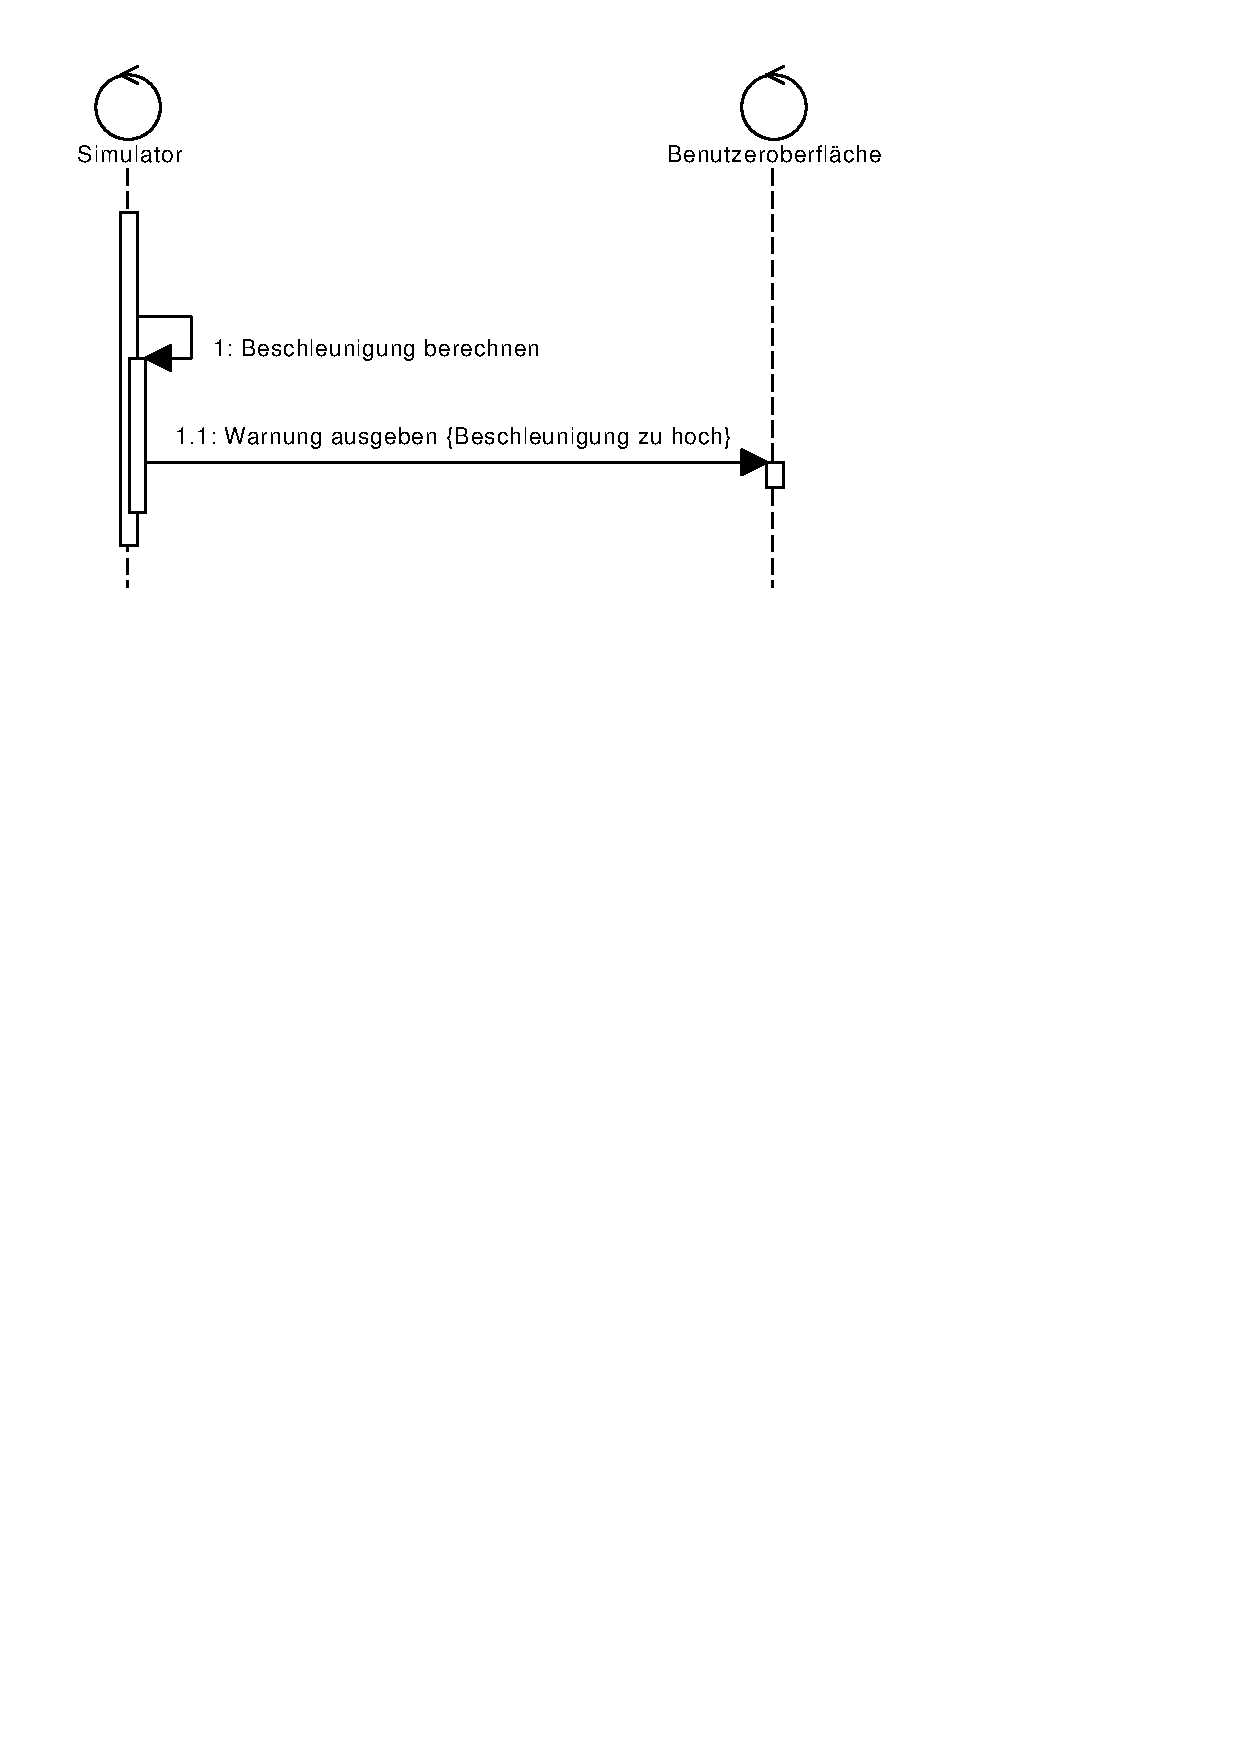
\includegraphics[width=\linewidth]{bilder/Warnung_Beschleunigung}
\caption{Warnung vor zu hoher Beschleunigung}
%\label{labelname}
\end{figure}
%Marco:
\section{Analyse von Funktionalität /F1100/ :  Erkennung von Veränderungen an der Ursprungsdatei}
Während der Laufzeit kann der Benutzer die Bahn mit dem Editor verändern.
Eine Veränderung der Ursprungsdatei wird erkannt und der Benutzer gefragt ob er die Bahn neu laden möchte oder weiter mit der aktuellen Bahn arbeiten will.
  % Kapitel 2
% Kapitel 3 mit den entsprechenden Unterkapiteln
% Die Unterkapitel können auch in separaten Dateien stehen,
% die dann mit dem \include-Befehl eingebunden werden.
%------------------------------------------------------------------------------------
\chapter{Resultierende Softwarearchitektur}

Dieses Kapitel erläutert die geplante Architektur des Achterbahnsimulators und
liefert eine grobe Spezifikation der Schnittstellen zwischen den geplanten
Komponenten.

\section{Komponentenspezifikation}

Aus der Analyse der Produktfunktionen ergeben sich sechs größere Teilbereiche,
die als Komponenten dieser Anwendung umgesetzt werden soll. Ersichtlich in Abbildung ~\ref{fig:component_overview}.

Im Kern der Anwendung steht die Simulator-Komponente, die für die Steuerung der
Achterbahnbewegung verantwortlich ist und zwischen der physikalischen Berechnung
und der grafischen Umsetzung koordiniert. Dieser Komponente wird von Außen die
Spezifikation einer Achterbahn übergeben, welche als Simulation umgesetzt werden
soll. Die Komponente hält über eine Endlosschleife (``render loop'') den Ablauf im Gang.

Die dreidimensionale Visualisierung der Achterbahn mit Gerüst und Umgebung wird
von der 3D-Anzeige-Komponente (``3D Graphics Engine'') übernommen. Sie kapselt die allgemeinen gehaltenen
Funktionen der eingesetzten Grafikbibliothek und stellt eine einfache Schnittstelle
für das Befüllen der virtuellen Welt mit Achterbahnkomponenten sowie zur Steuerung
der Kamerafahrten entlang der befahrenen Strecke zur Verfügung.

Die physikalische Berechnung der Achterbahnbewegung erfolgt in der Physik-Komponente
(``Physics'' Engine). Hier wird die Bewegung eines Massenpunktes auf der vorgegebenen Raumkurve
nach den Gesetzen der klassischen Mechanik durch Lösen einer gewöhnlichen 
Differentialgleichung bestimmt. Die berechnete Bahnkurve wird dem Simulator zur
Umsetzung der Kamerafahrt bereitgestellt.

Um die über Stützstellen definierte Achterbahn in eine ununterbrochene und hinreichend
glatte Raumkurve umzurechnen, kommt die Mathematik-Komponente (``Mathematics'') zum Einsatz. Im
Wesentlichen besteht die Komponente aus den Routinen zur näherungsweisen Berechnung
von Beziérkurven, dem Lösen von gewöhnlichen Differentialgleichungen (Anfangswertproblemen)
und Algorithmen zum Lösen von linearen Gleichungssystemen.

Für das Einlesen der Achterbahn-Spezifikationen aus den vom Editor bereitgestellten
XML-Dateien kommt die Dateiverwaltungs-Komponente (``File Management'') zum Einsatz. Diese kapselt alle
am speziellen Serialisierung-Schema haftenden Eigenheiten ab und liefert einen
von den anderen Komponenten einfach auslesbaren Datensatz mit dem Stützstellen der
Bahn und weiteren Parametern.

Die grafische Benutzeroberfläche (``Graphical User Interface'') übernimmt die Interaktion zwischen dem Benutzer und
der Simulation. Es übernimmt die Steuerung des Hauptmenüs, des Dateidialoges und
des Optionen-Dialogs. Die aus der Dateiverwaltung ausgelesenen Achterbahn-Datensätze 
werden an den Simulator zur Darstellung übergeben. Die Nutzeraktionen bezüglich des
Simulationsablaufes werden durchgereicht.

\begin{figure}
\includegraphics[width=\linewidth]{bilder/component_overview}
\caption{Komponentendiagramm für den Achterbahnsimulator}
\label{fig:component_overview}
\end{figure}

\section{Schnittstellenspezifikation}

Im Folgenden werden die einzelnen Schnittstellen der Komponenten aus der
Komponentenspezifikation näher erläutert, d. h. die von ihnen zur Verfügung
gestellten Operationen werden dokumentiert. Die Tabelle ist dabei um so viele
Zeilen zu erweitern, wie es Schnittstellen im Komponentendiagramm gibt. In der
innen liegenden Aufteilung ist für jede Operation einer Schnittstelle eine
Zeile einzufügen.  Reine Set- und Get-Aufrufe brauchen nicht aufgeführt zu
werden (sollten auch möglichst nicht komponentenübergreifend auftauchen).

\begin{tabular}[ht]{|l|p{0.35\linewidth}|p{0.35\linewidth}|}
 \hline
 Schnittstelle & \multicolumn{2}{|c|}{Aufgabenbeschreibung}\\
 \hline
 \hline
    /S10/ Track & \multicolumn{2}{|c|}{Spezifikation der Achterbahn mit Stützstellen und Parametern}\\
 \hline
 & getCurve() : Curve & Liefert die Achterbahnstrecke als mathematische Raumkurve zurück.\\ 
 \hline
    /S20/ Curve & \multicolumn{2}{|c|}{Repräsentation einer ortientierten Raumkurve}\\
 \hline
 & getLength() : double & Liefert die Länge der Raumkurve.\\ 
 & getPoint(lengh : double) : CurvePoint & Liefert den Repräsentanten für einen bestimmen Punkt auf der Raumkurve zurück,
 wobei über die Bogenlänge parametrisiert wird.\\ 
 & getPointSequence(maxDistance : double, maxAngle : double) : List<CurvePoint> &
 	Liefert eine Liste mit Punkten auf der Raumkurve wieder, die höchsten den angegebenen Abstand und die
 	Differenz im Raumwinkel haben dürfen. \\
 \hline
    /S21/ CurvePoint & \multicolumn{2}{|c|}{Repräsentation eines bestimmten Punktes auf einer Raumkurve}\\
 \hline
 & getPosition() : Vector & Liefert die Position. \\
 & getRollAxis() : Vector & Liefert die Rollachse (Längsachse).\\ 
 & getPitchAxis() : Vector & Liefert die Nickachse (Querachse). \\ 
 & getYawAxis() : Vector & Liefert die Gierachse (Hochachse). \\
 \hline
 	/S30/ Trajectory & \multicolumn{2}{|c|}{Bahnkurve des Massenpunktes über die Zeit}\\
 \hline
 & computeTimeStep(timeDiff : double) : void & Führt die Zeitentwicklung für den Massenpunkt durch. \\
 & getState() : TrajectoryPoint & Liefert den Zustand des Massenpunktes zum aktuellen Zeitpunkt zurück. \\
 \hline
 	/S31/ TrajectoryPoint & \multicolumn{2}{|c|}{Momentaufnahme des Massenpunktes auf der Bahnkurve}\\
 \hline
 & getPosition() : Vector & Liefert die Position.\\ 
 & getVelocity() : Vector & Liefert die Geschwindigkeit.\\ 
 & getAcceleration() : Vector & Liefert die Beschleunigung. \\ 
 & getJerk() : Vector & Liefert den Ruck. \\
 \hline
 \end{tabular}

\begin{tabular}[ht]{|l|p{0.35\linewidth}|p{0.35\linewidth}|}
 \hline
 Schnittstelle & \multicolumn{2}{|c|}{Aufgabenbeschreibung}\\
 \hline
 \hline
    /S40/ Simulation & \multicolumn{2}{|c|}{Repräsentant für eine konkrete Simulation}\\
 \hline
 & start() : void & Startet die Simulation.\\ 
 & stop() : void & Stoppt die Simulation. \\ 
\hline
	/S50/ View & \multicolumn{2}{|c|}{Repräsentant für die 3D-Welt mit bestimmter Kameraperspektive}\\
\hline
 & setCamera(positon : Vector, direction : Vector) & Setzt die Kamera auf die angegebene Position und Raumrichtung. \\ 
 \hline

 & setCurve(curve : Curve) & Setzt die Bahndaten, die zur Darstellung kommen sollen. \\ 
 \hline

 \end{tabular}





\section{Protokolle für die Benutzung der Komponenten}

%In diesem Abschnitt wird mit Hilfe von Protokoll-Statecharts die korrekte
%Verwendung der zu entwickelnden Komponenten dokumentiert. Dies ist insbesondere
%für diejenigen Komponenten notwendig, für die eine Wiederverwendung möglich
%erscheint oder sogar bereits geplant ist.

%Begründen Sie für welche Komponenten eine Wiederverwendung sinnvoll erscheint
%und für welche nicht!
Der Achterbahnsimulator setzt trotz seines (schon durch den Namen ersichtlichen)
eingeschränkten Anwendungsbereiches bereits alle wesentlichen Teile für die
Simulation anderer mechanischer Systeme um: die Berechnung der Bewegung von
Punktmassen wird auch ohne Einschränkung auf konkrete Kurven abgedeckt. Es liegt
deswegen nahe, diese Komponente sauber zu kapseln und wiederverwendbar zu gestalten.

Die Benutzeroberfläche ist eine konkret auf die Funktionalität der Anwendung
zugeschnittene Komponente. Allerdings dürfte die Oberfläche ohne größere
Schwierigkeiten auf andere Simulatoren neben Achterbahnen verallgemeinerbar sein.
Jede andere Art von Anwendung dürfte einen anderen Satz an Dialogfenstern und
Menübefehlen benötigen und andere Informationen auf dem Bildschirm darstellen,
so dass bei dieser Komponente ingesamt kein größerer Aufwand für eine
Wiederverwertung aufgebracht werden sollte.

Die 3D-Anzeige ist ebenfalls nicht auf bestimmte Modelle eingeschränkt, zumal in
der geplanten Architektur alle Dekorationen dynamisch zugefügt werden können.
Allerdings ist das zum Einsatz kommende 3D-Framework selber schon von sich aus 
für die Wiederverwertung ausgelegt, so dass der Mehrwert der eigenen Komponente
zumindest angezweifelt werden. Erst im Zusammenspiel mit dem Simulator und der 
Benutzeroberfläche erscheint der Mehraufwand für eine allgemeinere Schnittstelle
vertretbar.

Die Dateiverwaltung ist eine auf das Einlesen der vorgegebenen XML-Spezifikation 
zugeschnittene Spezialkomponente. Da der eingesetzte XML-Parser die Funktionalität
für allgemeine Fälle bereitstellt, scheint eine Wiederverwertung dieses Teils der
Anwendung nicht sinnvoll.

Alle mathematischen Routinen sollten selbstverständlich möglichst allgemein und
wiederverwertbar entworfen werden. Es muss nur sichergestellt werden, dass die
Implementierungen effizient bleiben.
      % Kapitel 3
% Kapitel 4
%-------------------------------------------------------------------------------
\chapter{Verteilungsentwurf}
4  Verteilungsentwurf
Sollte es sich bei dem Produkt um eine verteilte Anwendung handeln, so wird
diese in diesem Abschnitt dokumentiert. Die Verteilung der Komponenten auf die
beliebigen Knoten wird durch das folgende Verteilungsdiagramm beschrieben.



Eigenes Verteilungsdiagramm einsetzen!
        % Kapitel 4

%------Ende des Dokumentes------------------------------------------------------
\end{document}
